\documentclass[letterpaper]{article}
\title{Poaky documentation}
\author{Thomas HOULLIER} 

\usepackage[colorlinks=true, allcolors=blue,
            hyperfootnotes=false,
            pdfauthor={Thomas HOULLIER},
            pdftitle={Poaky documentation},
	    pdfkeywords={Optical design, Raytracing, C++}]
            {hyperref} % Links for ref/cite.

%% Loading packages
\usepackage{amsmath} % For cases in equations.
\usepackage{amsfonts} % For maths sets.
\usepackage{amssymb} % Square symbol for QED
\usepackage{physics} % For \abs{} and \norm{}.
\usepackage[inkscapelatex=false]{svg} %svg graphics
\usepackage{siunitx} % units formatting

\usepackage[backend=biber,style=numeric,citestyle=numeric-comp,maxcitenames=99,dateabbrev=false]{biblatex}
\addbibresource{biblio.bib}
\usepackage{setspace} % Bibliography spacings
\DeclareSourcemap{
  \maps[datatype=bibtex]{
    \map[overwrite]{
      \step[fieldsource=doi, final]
      \step[fieldset=url, null]
      \step[fieldset=eprint, null] }}}
\setcounter{biburllcpenalty}{7000} % break long url in bibliography
\setcounter{biburlucpenalty}{8000}
\renewcommand*{\bibfont}{\footnotesize} % bibliography font size
% Format of biblatex urldate in the bibliography.
\DeclareFieldFormat{urldate}{%
  Visited on \thefield{urlday}\addspace%
  \mkbibmonth{\thefield{urlmonth}}\addspace%
  \thefield{urlyear}\isdot}
\usepackage[ruled,vlined]{algorithm2e} % Algorithms.
\DontPrintSemicolon
\SetKwInOut{Input}{Input}\SetKwInOut{Output}{Output}
\usepackage{mathtools} % Ceiling function.
\usepackage{outlines} % Nest lists.
\usepackage{interval} % Writing intervals.
\usepackage[font={footnotesize,sf}]{caption} %Caption for figures in minipages.
\usepackage{floatrow}
% Figure captions always below. Figures always centered.
\floatsetup[figure]{capposition=bottom,objectset=centering}
\usepackage{wrapfig} %Wrapping figure with text.
\usepackage{stmaryrd} % Double brackets for integers interval.
\usepackage{doi} % Hyperlink DOI
\usepackage{etoolbox} %Ragged right bibliography.
\usepackage{color, colortbl} % Coloring rows in tables.
\usepackage{subcaption} % Subfigures.
\usepackage{pdfpages} % Include PDF pages.
\usepackage{epigraph} % Quotations at beginning of chapters.
\usepackage[en-GB]{datetime2} % Dates formatting
\DTMlangsetup{abbr,ord=omit,monthyearsep={\space}}
\setlength\epigraphwidth{.8\textwidth}
\usepackage[acronym,nonumberlist,nogroupskip,nopostdot]{glossaries} % Glossary for acronyms.
\renewcommand*{\glstextformat}[1]{\textcolor{black}{#1}} % No color on links for abbrev.

\DeclarePairedDelimiter{\ceil}{\lceil}{\rceil} % Ceiling function.
\DeclarePairedDelimiter{\floor}{\lfloor}{\rfloor} % Floor function.

\DeclareMathOperator*{\argmin}{argmin}

\setcounter{tocdepth}{3} % Table of content depth
\setcounter{secnumdepth}{3} % Section numbering depth

% Non-breaking around footnotes.
\makeatletter
\let\Footnote\footnote
\def\pst@@killglue{\unskip\ifdim\lastskip>\z@\expandafter\pst@@killglue\fi}
\def\footnote{\pst@@killglue\Footnote}
\makeatother

% More space below equations
\appto\normalsize{\belowdisplayshortskip=\belowdisplayskip}

% Rewrite month codes in bibliography
\DeclareSourcemap{
  \maps[datatype=bibtex]{
    \map[overwrite]{
      \step[fieldsource=month, match=\regexp{\A(j|J)an(uary)?\Z}, replace=1]
      \step[fieldsource=month, match=\regexp{\A(f|F)eb(ruary)?\Z}, replace=2]
      \step[fieldsource=month, match=\regexp{\A(m|M)ar(ch)?\Z}, replace=3]
      \step[fieldsource=month, match=\regexp{\A(a|A)pr(il)?\Z}, replace=4]
      \step[fieldsource=month, match=\regexp{\A(m|M)ay\Z}, replace=5]
      \step[fieldsource=month, match=\regexp{\A(j|J)un(e)?\Z}, replace=6]
      \step[fieldsource=month, match=\regexp{\A(j|J)ul(y)?\Z}, replace=7]
      \step[fieldsource=month, match=\regexp{\A(a|A)ug(ust)?\Z}, replace=8]
      \step[fieldsource=month, match=\regexp{\A(s|S)ep(tember)?\Z}, replace=9]
      \step[fieldsource=month, match=\regexp{\A(o|O)ct(ober)?\Z}, replace=10]
      \step[fieldsource=month, match=\regexp{\A(n|N)ov(ember)?\Z}, replace=11]
      \step[fieldsource=month, match=\regexp{\A(d|D)ec(ember)?\Z}, replace=12]}}}

% Footnotes marker color
\renewcommand\thefootnote{\textcolor{blue}{\arabic{footnote}}}

\pdfsuppresswarningpagegroup=1 % Silence warnings about pagegroups for figures.
\pdfminorversion=6 % PDF version 1.6 since we include articles in 1.6.

% Allow an extra pass to fix overfull hboxes by allowing more whitespace.
\emergencystretch=1em

% Page numbering and copyright notice.
\usepackage{fancyhdr}
\usepackage{lastpage}

\fancypagestyle{FirstPage}{
\fancyhf{} % Clear footer.
\rfoot{\thepage \hspace{1pt} of \pageref*{LastPage}}
\renewcommand{\headrulewidth}{0pt} % Remove rule at top of page
\lfoot{\href{https://creativecommons.org/licenses/by/4.0/}
       {\includesvg[inkscapelatex=false,height=14pt]{images/ccby.svg}}}
\lhead{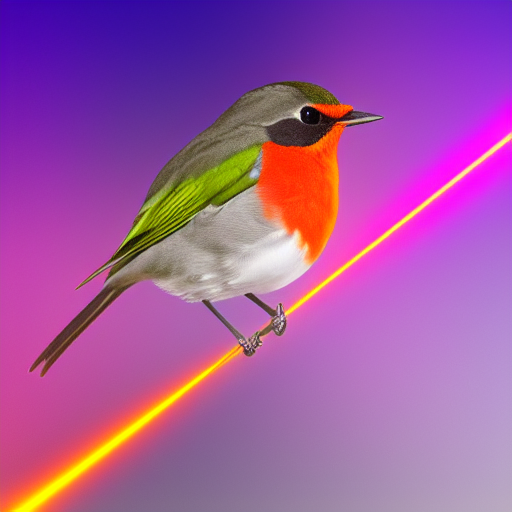
\includegraphics[height=64pt]{images/robintrace-logo.png}}
\chead{RobinTrace}
}

\fancypagestyle{plain}{
\fancyhf{} % Clear footer.
\rfoot{\thepage \hspace{1pt} of \pageref*{LastPage}}
\renewcommand{\headrulewidth}{0pt} % Remove rule at top of page
}

% Version history
\usepackage{vhistory}

% Keywords
\providecommand{\keywords}[1]{\textbf{Keywords --} #1}

% Glossary
\makeglossaries
\loadglsentries{glossary/glossary.tex}

\usepackage{fontawesome} %inline icons
\usepackage{xcolor}
\usepackage{listings} % Code listings
\definecolor{codeback}{rgb}{0.99,0.99,0.98}
\definecolor{codecomment}{HTML}{0588fc}
\definecolor{codekeyword}{HTML}{af5f00}
\definecolor{codestring}{HTML}{ffa07a}
\lstdefinestyle{mystyle}{
  backgroundcolor=\color{codeback},
  commentstyle=\color{codecomment},
  keywordstyle=\color{codekeyword},
  stringstyle=\color{codestring},
  basicstyle=\ttfamily\footnotesize,
  breakatwhitespace=false,         
  breaklines=true,                 
  captionpos=b,                    
  keepspaces=true,                 
  numbers=left,                    
  numbersep=5pt,                  
  showspaces=false,                
  showstringspaces=false,
  showtabs=false,                  
  tabsize=2}
\lstset{style=mystyle}

\usepackage[capitalise,nameinlink]{cleveref} % Include eg. "Fig." in front of figures.
\crefname{algorithm}{Alg.}{Algs.}
\crefname{table}{Tab.}{Tabs.}
\crefname{equation}{Eq}{Eqs.}
% Equation cross-references.
%\creflabelformat{equation}{#2#1#3}
\crefformat{equation}{(#2Eq.\thinspace#1#3)}

% No parentheses in equation labels.
%\newtagform{noparen}{}{}
%\usetagform{noparen}



\begin{document}
\frenchspacing
\date{v1.0 -- \today}
\maketitle
\thispagestyle{FirstPage}

\begin{abstract}
Poaky is a low-level software API layer for RobinTrace. Poaky is a
reference implementation for ray-wise and element-wise operations in
the forward simulation of sequential raytracing. The software is
written in C++.
\end{abstract}

\keywords{Optical design, Sequential raytracing, C++}

\begin{versionhistory}
\vhEntry{1.0}{\today}{TH}{creation}
\end{versionhistory}
\setcounter{table}{0} % Reset the table counter.

\tableofcontents
\pagestyle{plain}

\section{Introduction}
We document Poaky, which is a software component of RobinTrace. Poaky deals
with basic ray-wise and element-wise sequential raytracing operations. Its
goal is to provide a reference implementation and document clearly the
forward simulation pass of sequential raytracing. The simulation is carried
out within the context of geometrical optics.

We had similar endeavours in a previous work \cite{Houllier-thesis}.
The present software is a rewrite of this work after putting more thought and
research into the problem. Much of the present work is ultimately a rehash of
the work of Welford \cite{Welford:1986}, who was foundational in computerized
optical design raytracing.

In its present version, only a handful of operations are implemented. The
current development goal is to reach a minimal working example in RobinTrace.
Whether Poaky will serve as the base layer for RobinTrace in its current state
or merely as a reference is not yet decided.

\section{Definitions and conventions}
We outline the conventions we use. Some details may differ from the choices
made in other tools.

\subsection{Raytracing sequence}
Poaky deals with the elementary operations in optical systems represented as a
sequence of objects operating on rays of light. The objects are of
two main types, optical surfaces and geometric propagators through some medium
in between surfaces (which we call \emph{transfer}). The sequence in which rays
of light interact with either surfaces or transfers is known a priori. The
simulation of the propagation of rays through such a sequence of objects is
known as \emph{sequential raytracing}. This discipline is linked with the more
well known raytracing for rendering, though they seem to have developed more or
less autonomously.

\subsection{Local coordinate system} \label{sec:LCS}
Each surface corresponds to an implicit \gls{LCS}.
This coordinate system may be described as containing (\cref{fig:LCS}):

\begin{itemize}
\item An apex $A$, which is the origin.
\item A local $z=0$ plane, which we often refer to as the \emph{local plane}.
\item A set of axes (implicit).
\end{itemize}

\begin{figure} \caption{\label{fig:LCS} LCS diagram.}
\includesvg[height=.2\textheight, width=.9\textwidth, keepaspectratio]
           {images/conventions/LCS.svg}
\end{figure}

We call the \gls{LCS} implicit because the actual meaning of the data
expressed in it depends on the interplay between surface defition, ray
transfer equations and ray operation conventions.

\subsection{Rays in local coordinate systems}

\begin{figure} \caption{\label{fig:ray-in-LCS} Ray definition
in \gls{LCS}.}
\includesvg[height=.2\textheight, width=.9\textwidth, keepaspectratio]
           {images/conventions/ray_in_LCS.svg}
\end{figure}

Given a \gls{LCS}, a ray may be defined by (\cref{fig:ray-in-LCS}):
\begin{itemize}
\item $P = \begin{bmatrix}x \\ y \\ z \end{bmatrix}$, a point.
\item $\overrightarrow{V} = \begin{bmatrix} l \\ m \\ n \end{bmatrix}$, a unit
vector oriented by the light propagation.
\end{itemize}

The components of $\overrightarrow{V}$ are often called in optics by the name
\emph{direction cosines} \cite{mathworld:direction-cosine}. Indeed, given the
basis vectors of our \gls{LCS}: $(\hat{x}, \hat{y}, \hat{z})$, the vector
$\overrightarrow{V}$ can be described by the angles $(\alpha, \beta, \gamma)$
between itself and each basis vector respectively. These angles may be defined
by \cref{eq:direction-cosines}.

\begin{equation} \label{eq:direction-cosines}
\begin{cases}
l &= \cos(\alpha) = \frac{\overrightarrow{V} \cdot \hat{x}}
                          {\abs{\overrightarrow{V}}} \\
m &= \cos(\beta) = \frac{\overrightarrow{V} \cdot \hat{y}}
                         {\abs{\overrightarrow{V}}} \\
n &= \cos(\gamma) = \frac{\overrightarrow{V} \cdot \hat{z}}
                          {\abs{\overrightarrow{V}}}
\end{cases}
\end{equation}

The points $(x_t, y_t, z_t)$ describing the ray trajectory through the use of a parameter $t$
are described by \cref{eq:ray-trajectory}.

\begin{equation} \label{eq:ray-trajectory}
\begin{bmatrix}
x_t \\ y_t \\ z_t
\end{bmatrix} =
\begin{bmatrix}
x + t \cdot l \\
y + t \cdot m \\
z + t \cdot n
\end{bmatrix}
\end{equation}

\section{Functional description}
\textcolor{red}{TODO: Remove the purely API descriptions from this section.}

This section defines the program's objects and their associated
operations. The style is minimal and close to the computations. For
the rationale sustaining the computation and complementary information,
see the justification section (\cref{sec:justification}).

\subsection{base}
Some base types are useful throughout the program. These are detailed in this
section.

\paragraph{Vec3}
\lstinline{Vec3} $\in \mathbb{R}^3$ are vectors in 3D space. They may
represent points or directions. Depending on the context, they can be
implicitely considered to have unit norm.

\paragraph{Mat3}
\lstinline{Mat3} $\in \mathbb{R}^{3 \times 3}$ are 3D matrices. They
are used to represent rotation matrices.

\subsection{ray}
\lstinline{ray} objects are the centerpiece of the simulation. They must be
lightweight objects.  \lstinline{ray} holds a position and a unit vector in the
direction and orientation of the propagation of light:

\begin{itemize}
\item \lstinline{Vec3 p}: A point.
\item \lstinline{Vec3 v}: A unit vector, oriented by light propagation.
\end{itemize}

The interpretation of the data contained in a \lstinline{ray} is dependent
on the context, as they are expressed in a given \gls{LCS}.

In addition to their geometric definition, rays also hold a status code.
This code signals whether raytracing operations were successful, and if
not, which error case was encountered. There is no guarantee on the value
of the ray point and vector when the status code signals an error.

\begin{itemize}
\item \lstinline{int code}: Status code.
\end{itemize}

The status codes are defined in \cref{tab:ray-status-codes}.

\begin{table} \caption{\label{tab:ray-status-codes} Ray status codes.}
\begin{tabular}{| c | l |} \hline
\textbf{Code} & \textbf{Meaning} \\ \hline
0 & Success, the ray is valid.\\ \hline
3 & refract: \gls{TIR} \\ \hline
4 & transfer: ray is parallel to the new local plane. \\ \hline
5 & standard intersection: No intersection. \\ \hline
\end{tabular} \end{table}

\subsection{rop}
\lstinline{rop} are ray operations.

\subsubsection{reflect}
\lstinline{reflect} is a ray operation which applies the law of specular
reflection \cite{wiki:specular-reflection}. The normal vector
$\overrightarrow{N}$ is an input to the operation. There are no error cases. The
operation is illustrated on \cref{fig:reflect}.

\begin{equation}
\begin{bmatrix} l_r \\ m_r \\ n_r \end{bmatrix} =
\begin{bmatrix} l \\ m \\ n \end{bmatrix} - 2 \cdot
\overrightarrow{N} \cdot \left( \overrightarrow{N} \cdot
\begin{bmatrix} l \\ m \\ n \end{bmatrix} \right)
\end{equation}

\begin{figure} \caption{\label{fig:reflect} reflect operation quantities.}
\includesvg[height=.2\textheight, width=.9\textwidth, keepaspectratio]
           {images/shape/abstract-reflect.svg}
\end{figure}

\subsubsection{refract}
\lstinline{refract} is a ray operation applying the Snell law of refraction
\cite{wiki:snell-refraction}. We use Xavier Bec's formula (\cite{Marrs:2021}
p.105, \cite{Bec:1997}) for efficiency.  The operation is illustrated on
\cref{fig:refract}.

\begin{figure} \caption{\label{fig:refract} refract operation quantities.}
\includesvg[height=.2\textheight, width=.9\textwidth, keepaspectratio]
           {images/shape/abstract-refract.svg}
\end{figure}

Let,

\begin{itemize}
\item $n_1$ the incident medium refraction index,
\item $n_2$ the output medium refraction index,
\item $n_r = \frac{n_1}{n_2}$,
\item $\overrightarrow{i}$ the unit incident ray direction,
\item $\overrightarrow{N}$ the unit surface normal vector,
\item $\overrightarrow{t}$ the unit refracted ray direction.
\end{itemize}

\begin{equation}
\begin{split}
&c_1 = - \overrightarrow{i} \cdot \overrightarrow{N} \\
&w = n_r \cdot c_1 \\
&c_{2m} = (w - n_r) \cdot (w + n_r)
\end{split} \end{equation}

At this stage, if $c_{2m} < -1$, then we set the \gls{TIR} ray
error code and the computation stops. Otherwise we proceed with
the computation of the refracted ray direction.

\begin{equation} \label{eq:bec-formula}
\overrightarrow{t} = n_r \cdot \overrightarrow{i} +
(w - \sqrt{1 + c_{2m}}) \cdot \overrightarrow{N}
\end{equation}

\subsection{transfer} \label{sec:transfer}
A transfer defines a new \gls{LCS} to propagate the ray to.  The transfer
operation a change of basis and an intersection with the newly defined
local plane.

\paragraph{Definition}
Let,
\begin{itemize}
\item LCS1 the starting \gls{LCS} defined by its origin and basis vectors
$(A_1, \hat{x_1}, \hat{y_1}, \hat{z_1})$,
\item LCS2 the \gls{LCS} defined by the transfer operation, 
$(A_2, \hat{x_2}, \hat{y_2}, \hat{z_2})$.
\end{itemize}

The transfer operation is characterized by
\begin{itemize}
\item \lstinline{Mat3} $B$: A rotation matrix between the basis vectors of LCS1
and LCS2. $B$ is orthogonal by definition, hence $B^{-1} = B^\top$
\cite{wiki:rotation-matrix}.
\item \lstinline{Vec3} $\overrightarrow{D}$: A translation vector between
LCS1 and LCS2.
\end{itemize}

The coordinates of the origin and basis vectors of LCS2 are expressed in
the original LCS1 coordinates by the following relations.

\begin{equation} \begin{cases}
A_2 = B \cdot \overrightarrow{D} \\
\hat{x_2} = B \cdot \hat{x_1} \\
\hat{y_2} = B \cdot \hat{y_1} \\
\hat{z_2} = B \cdot \hat{z_1}
\end{cases} \end{equation}

Which is to say, LCS2 is obtained from LCS1 by first applying the rotation $B$
and then translating the origin by $\overrightarrow{D}$, with
$\overrightarrow{D}$ expressed in the rotated coordinates. The change of basis
is illustrated on \cref{fig:transfer-definition}.

\begin{figure} \caption{\label{fig:transfer-definition}
Definition of the transfer between LCS1 and LCS2.}
\includesvg[height=.2\textheight, width=.9\textwidth, keepaspectratio]
           {images/shape/transfer-definition.svg}
\end{figure}

\paragraph{Operation}
The \lstinline{transfer} operation can be decomposed as two successive
operations on the ray:

\begin{itemize}
\item A change of basis from LCS1 to LCS2.
\item A ray intersection with the local plane of LCS2.
\end{itemize}

Let a ray expressed in LCS1 with starting point and direction
$(P_1, \overrightarrow{V_1})$. We first operate a change of basis from LCS1
to LCS2, which gives the coordinates $(P_2, \overrightarrow{V_2})$.

\begin{equation} \begin{cases}
P_2 = \begin{bmatrix} x_2 \\ y_2 \\ z_2 \end{bmatrix}
    = B^{-1} \cdot P_1 - \overrightarrow{D} \\
\overrightarrow{V_2} = \begin{bmatrix} l_2 \\ m_2 \\ n_2 \end{bmatrix}
  = B^{-1} \cdot \overrightarrow{V_1}
\end{cases} \end{equation}

We signal an error in the case $n_2 = 0$. This case corresponds to the
ray being parallel to the local plane of LCS2. We operate the intersection
of the ray with the LCS2 local plane next. The result ray is
$(P_3, \overrightarrow{V_3})$. The operation is illustrated by
\cref{fig:transfer-operation}.

\begin{equation} \begin{cases}
\overrightarrow{V_3} = \overrightarrow{V_2} \\
t = - \frac{z_2}{n_2} \\
P_3 = \begin{bmatrix} x_2 + t \cdot l_2 \\
                      y_2 + t \cdot m_2 \\
                      0 \end{bmatrix}
\end{cases} \end{equation}

\begin{figure} \caption{\label{fig:transfer-operation}
Illustration of the transfer operation on a ray.}
\includesvg[height=.2\textheight, width=.9\textwidth, keepaspectratio]
           {images/shape/transfer-operation.svg}
\end{figure}

\subsection{shape}
Shape is an abstract concept specifying two operations:

\begin{itemize}
\item \lstinline{intersect}: Intersect a ray with the shape.
\item \lstinline{normal}: Provide a vector normal to the shape at the current
      ray position.
\end{itemize}

\paragraph{intersect}
The intersection operation takes a \lstinline{ray} expressed in the current
surface coordinate system with point on the local plane. It computes the
intended intersection point between the ray and the shape.  This operation is
illustrated on \cref{fig:abstract-rayinter}.

\begin{figure} \caption{\label{fig:abstract-rayinter} Illustration of the
abtract intersect operation for a shape on a ray.}
\includesvg[height=.2\textheight, width=.9\textwidth, keepaspectratio]
           {images/shape/abstract-rayinter.svg}
\end{figure}

\paragraph{normal}
The normal operation provides a normal vector at the ray's current
position on the shape. The normal vector is expressed in the surface
LCS. The normal vector is a unit vector. The normal vector is oriented
with a $\hat{z}$ component of opposite sign to that of the ray's vector,
\textit{ie} the normal vector is in the opposite half-plane to the incident
ray. The normal operation is illustrated on \cref{fig:abstract-normal}.

\begin{figure} \caption{\label{fig:abstract-normal} Illustration of the
abstract normal operation for a shape and a ray.}
\includesvg[height=.2\textheight, width=.9\textwidth, keepaspectratio]
           {images/shape/abstract-normal.svg}
\end{figure}

\subsubsection{plane}
\paragraph{Definition}
A \lstinline{plane} is the local $z=0$ plane in the current \gls{LCS}.
It is specified implicitely.

\paragraph{intersect}
The input ray is already on the local plane. We do \emph{nothing} and cannot
fail.

\paragraph{normal}
The plane normal vector is trivial.
It is $\overrightarrow{N} = (0, 0, -\textrm{sign}(n))$.
There are no error cases.

\subsubsection{standard}
The so-called \lstinline{standard} shape describes surfaces which
belong to quadrics of revolution with axis $z$.

\paragraph{Definition}
The surface shape \lstinline{standard} is defined using:
\begin{itemize}
\item $c$: the radius of curvature reciprocal, $c = \frac{1}{R}$.
\item $k$: a scalar parameter which changes the type of the quadric.
\end{itemize}

The mathematical classification of the surface depends on the value of
$k$,

\begin{itemize}
\item $k < -1$: One of the sheets of a hyperboloid of revolution of two sheets.
\item $k = -1$: Circular paraboloid.
\item $k > -1$: Spheroid, with the case $k=0$ being a sphere.
\end{itemize}

Note that the case $c=0$ describes a plane.

An explicit altitude formula may be given for part of the surface (in the case
of spheroids, only the hemisphere containing the apex is described by this
formula). Let $r^2 = x^2 + y^2$.

\begin{equation} \label{eq:standard-z}
z = \frac{c \cdot r^2}{1 + \sqrt{1 - (k + 1) \cdot c^2 \cdot r^2}}
\end{equation}

The effective surface definition is given by the \lstinline{intersect}
operation.  Please note that in the case of spheroids, intersections
beyond the hemisphere closest to the apex are valid.

\paragraph{intersect}
The intersection point $I$ is found with the following operations sequence.

\begin{equation} \begin{cases}
f = c \cdot ({x_P}^2 + {y_P}^2) \\
g = n - c \cdot (l \cdot x_P + m \cdot y_P) \\
h = g^2 - c \cdot f \cdot (1 + k \cdot n^2)
\end{cases} \end{equation}

In the case $h \leq 0$, we signal a ray error of absence of intersection.
Else we continue,

\begin{equation}
t = \frac{f}{g + \textrm{sign}(n) \cdot \sqrt{h}}
\end{equation}

\begin{equation}
I = \begin{bmatrix} x_P \\ y_P \\ 0 \end{bmatrix} + t \cdot
    \begin{bmatrix} l \\ m \\ n \end{bmatrix}
\end{equation}

\paragraph{normal}
The normal vector at the current point is given by,

\begin{equation}
\overrightarrow{N} =
\begin{bmatrix}
c \cdot x \\ c \cdot y \\ c \cdot (k+1) \cdot z - 1
\end{bmatrix} \cdot
\frac{\textrm{sign}(n)}{
\sqrt{1 - 2 c \cdot k \cdot z + c^2 \cdot (k+1) \cdot k \cdot z^2}}
\end{equation}


\section{Proofs and justification}
\label{sec:justification}

Some implementation details require further justification and explanations.
The mathematical derivations are written with sufficient details so that
they may be followed without pen and paper.

\subsection{Ray operations (rop)}
Various formulae derivations and checks are presented.

\subsubsection{Reflection formula derivation}
We derive the reflection formula. See the illustration \cref{fig:reflect}.
Let: \begin{itemize}
\item The surface normal $\overrightarrow{N}$ at the ray intersection.
\item The incident ray unit vector $\overrightarrow{i}$.
\item The reflected ray unit vector $\overrightarrow{r}$.
\item $\theta_i$ the (unsigned) angle between $\overrightarrow{N}$ and
      $\overrightarrow{i}$.
\item $\theta_r$ the (unsigned) angle between $\overrightarrow{N}$ and
      $\overrightarrow{r}$.
\end{itemize}

We want to compute $\overrightarrow{r}$ as a function of $\overrightarrow{i}$
and $\overrightarrow{N}$.  We assume the laws of reflection, which essentially
state that light behaves as a billiard ball in its geometrical interaction with
the surface.  We present several ways of looking at the problem. In our
opinion, these are not so much derivations as different restatements of the
laws of reflection.

\paragraph{Bounce derivation}
The effect of the light bouncing off the surface can be stated in the following
fashion. The component of $\overrightarrow{i}$ colinear to $\overrightarrow{N}$
is inverted by the reflection. The other components of $\overrightarrow{i}$ stay
the same. This immediately gives the tractable relation.

\begin{equation}
\overrightarrow{r} = \overrightarrow{i} - 2 \cdot (\overrightarrow{N} \cdot
\overrightarrow{i}) \cdot \overrightarrow{N}
\end{equation}

\paragraph{Geometric construction}
The ray reflection may be viewed as a geometric construction based on the
laws of reflection (see \cite{Glassner:1989} p.291 \cite{Comninos:2010}
p.335). We draw the geometric view of the problem on
\cref{fig:reflect-geometry}.

\begin{figure} \caption{\label{fig:reflect-geometry} Illustration for the
geometric construction of the reflect operation.}
\includesvg[height=.2\textheight, width=.9\textwidth, keepaspectratio]
           {images/shape/reflect-geometry.svg}
\end{figure}

\paragraph{Algebraic derivation}
We produce a derivation similar to the one included in \cite{Glassner:1989}
(p.131).

\begin{itemize}
\item The reflected ray is in the plane spanned by $\overrightarrow{i}$ and
      $\overrightarrow{N}$ (\emph{plane of incidence}).
\item $\theta_i = \theta_r$
\item Except in the degenerate case $\overrightarrow{i} = - \overrightarrow{N}$,
$\overrightarrow{r} \neq - \overrightarrow{i}$. Ie the reflected ray does not
retrace on the incident ray.
\end{itemize}

Translated algebraically, these statements suffice to determine a formula for
$\overrightarrow{r}$. Let $(\alpha, \beta)$ both in $\mathbb{R}$. The reflected
ray in the incidence plane must be expressed as:

\begin{equation}
\overrightarrow{r} = \alpha \cdot \overrightarrow{i} +
                     \beta \cdot \overrightarrow{N}
\end{equation}

We now add the remaining constraints on $\overrightarrow{r}$ in order to narrow
down expressions for $\alpha$ and $\beta$.

\begin{equation} \begin{split}
& \theta_i = \theta_r \\
\implies & \cos(\theta_i) = \cos(\theta_r) \\
\implies & - \overrightarrow{i} \cdot \overrightarrow{N} =
       \overrightarrow{N} \cdot \overrightarrow{r}
\end{split} \end{equation}

\begin{equation} \begin{split}
- \overrightarrow{i} \cdot \overrightarrow{N} &=
\overrightarrow{N} \cdot
(\alpha \cdot \overrightarrow{i} + \beta \cdot \overrightarrow{N}) \\
&= \alpha \cdot \overrightarrow{i} \cdot \overrightarrow{N} +
   \beta \cdot \overrightarrow{N} \cdot \overrightarrow{N} \\
&= \alpha \cdot \overrightarrow{N} \cdot \overrightarrow{i} + \beta
\end{split} \end{equation}

Hence the following expression for $\beta$.

\begin{equation} \label{eq:reflect-beta-expr}
\beta = - (\alpha + 1) \cdot \overrightarrow{N} \cdot \overrightarrow{i}
\end{equation}

Another constraint we exploit is that $\overrightarrow{r}$ is a unit vector.

\begin{equation} \begin{split}
& \abs{\overrightarrow{r}} = 1 \\
\implies& \abs{\alpha \cdot \overrightarrow{i} +
                \beta \cdot \overrightarrow{N}} = 1 \\
\implies& (\alpha \cdot i_x + \beta \cdot N_x)^2 +
          (\alpha \cdot i_y + \beta \cdot N_y)^2 +
          (\alpha \cdot i_z + \beta \cdot N_z)^2 = 1 \\
\implies& \alpha^2 ({i_x}^2 + {i_y}^2 + {i_z}^2) +
          \beta^2 ({N_x}^2 + {N_y}^2 + {N_z}^2) + \\
          &2 \cdot \alpha \cdot \beta 
          (i_x \cdot N_x + i_y \cdot N_y + i_z \cdot N_z) = 1 \\
\implies& \alpha^2 + \beta^2 + 2 \cdot \alpha \cdot \beta \cdot
          \overrightarrow{N} \cdot \overrightarrow{i} = 1
\end{split} \end{equation}

Now we plug the expression for $\beta$ \cref{eq:reflect-beta-expr}.

\begin{equation} \begin{split}
\implies& \alpha^2 + (\alpha + 1)^2
(\overrightarrow{N} \cdot \overrightarrow{i})^2
- 2 \cdot \alpha (\alpha + 1) \cdot
(\overrightarrow{N} \cdot \overrightarrow{i})^2 = 1 \\
\implies& \alpha^2 (1 - 2 (\overrightarrow{N} \cdot \overrightarrow{i})^2
+ (\overrightarrow{N} \cdot \overrightarrow{i})^2) + \\
& \alpha (-2\cdot (\overrightarrow{N} \cdot \overrightarrow{i})^2
        +2 \cdot (\overrightarrow{N} \cdot \overrightarrow{i})^2) +
(\overrightarrow{N} \cdot \overrightarrow{i})^2 = 1 \\
\implies& \alpha^2 \cdot (1 - (\overrightarrow{N} \cdot \overrightarrow{i})^2)
+ (\overrightarrow{N} \cdot \overrightarrow{i})^2 = 1 \\
\implies& \alpha^2 = \frac{1 - (\overrightarrow{N} \cdot \overrightarrow{i})^2}
                          {1 - (\overrightarrow{N} \cdot \overrightarrow{i})^2}
\end{split} \end{equation}

The degenerate case $\overrightarrow{i} = - \overrightarrow{N}$, which
leads to $1 - (\overrightarrow{N} \cdot \overrightarrow{i})^2 = 0$, is excluded.
The answer in the degenerate case is $\overrightarrow{r} = -
\overrightarrow{i}$. We continue the main derivation path with:

\begin{equation}
\alpha = \pm 1
\end{equation}

The case $\alpha = -1$ leads to $\beta = 0$ and $\overrightarrow{r} = -
\overrightarrow{i}$. We excluded this case by hypothesis.  The remaining answer
is $\alpha = + 1$.

Summarizing:

\begin{equation} \begin{cases}
\alpha = 1 \\
\beta = -2 \cdot \overrightarrow{N} \cdot \overrightarrow{i}
\end{cases} \end{equation}

This leads us to the expression for $\overrightarrow{r}$.

\begin{equation}
\overrightarrow{r} = \overrightarrow{i} - 2 \cdot (\overrightarrow{N} \cdot
\overrightarrow{i}) \cdot \overrightarrow{N}
\end{equation}

$\square$

\subsubsection{Refraction}
We derive the refraction formula vectorial form from the laws of refraction.
Then we check the equivalence of Bec's formula with the derived refraction
formula.

\paragraph{Algebraic derivation}
We work through an algebraic derivation of the vectorial expression for
the refraction operation. Similar derivations may be found in
\cite{Glassner:1989} (p.288), originally by Whitted \cite{Whitted:2005}
and Heckbert \cite{Heckbert:1984}.

The quantities involved in the problem are (illustrated on
\cref{fig:refract-derivation}):

\begin{itemize}
\item $n_1$ the incident medium refraction index,
\item $n_2$ the output medium refraction index,
\item $\overrightarrow{i}$ the unit incident ray direction,
\item $\overrightarrow{N}$ the unit surface normal vector,
\item $\overrightarrow{t}$ the unit refracted ray direction,
\item $\theta_i$ the acute angle between $-\overrightarrow{i}$
and $\overrightarrow{N}$,
\item $\theta_t$ the angle between $-\overrightarrow{N}$ and
$\overrightarrow{t}$.
\end{itemize}

\cref{fig:refract-derivation}
\begin{figure} \caption{\label{fig:refract-derivation} Quantities involved
in the ray refraction operation.}
\includesvg[height=.2\textheight, width=.9\textwidth, keepaspectratio]
           {images/shape/refract-derivation.svg}
\end{figure}

We take for granted a number of assumptions related to the law of refraction
\cite{wiki:snell-refraction}:

\begin{itemize}
\item $\overrightarrow{t}$ is in the plane spanned by $\overrightarrow{i}$
and $\overrightarrow{N}$ (\emph{plane of incidence}),
\item Defining quadrants in the plane of incidence with respect to
$\overrightarrow{N}$ and the origin, $\overrightarrow{t}$ is in
the same quadrant as $\overrightarrow{i}$,
\item $n_1 \cdot \sin(\theta_i) = n_2 \cdot \sin(\theta_t)$
\item In the particular case where $-\overrightarrow{i} = \overrightarrow{N}$,
      the refracted ray is $\overrightarrow{t} = - \overrightarrow{N}$.
\end{itemize}

We remind some relations and define some shorthands used for conciseness.

\begin{equation} \begin{cases}
- \overrightarrow{N} \cdot \overrightarrow{i} = \cos(\theta_i) = c_i \\
- \overrightarrow{N} \cdot \overrightarrow{t} = \cos(\theta_t) = c_t \\
\sin(\theta_i) = s_i \\
\sin(\theta_t) = s_t \\
\frac{n_1}{n_2} = n_r
\end{cases} \end{equation}

Since $\overrightarrow{t}$ is in the incidence plane, it may be written as:

\begin{equation}
\overrightarrow{t} = \alpha \cdot \overrightarrow{i}
                     + \beta \cdot \overrightarrow{N}
\end{equation}

The other hypotheses provide the following constraints, which we will use
in order to solve for $\alpha$ and $\beta$.

\begin{equation} \begin{cases}
n_1 \cdot s_i = n_2 \cdot s_t \\
\abs{\overrightarrow{t}} = 1
\end{cases} \end{equation}

We may express a relation with the help of $c_t$:

\begin{equation} \begin{split}
c_t &= - \overrightarrow{N} \cdot \overrightarrow{t} \\
&= - \overrightarrow{N} \cdot
   (\alpha \cdot \overrightarrow{i} + \beta \cdot \overrightarrow{N}) \\
&= - \alpha \cdot \overrightarrow{N} \cdot \overrightarrow{i} - \beta \\
&= \alpha \cdot c_i - \beta
\end{split} \end{equation}

Thus,

\begin{equation}
\beta = \alpha \cdot c_i - c_t
\end{equation}

The $\overrightarrow{t}$ normalization constraint gives us another expression:

\begin{equation} \begin{split}
\abs{\overrightarrow{t}} &= \abs{\alpha \cdot \overrightarrow{i}
                                 + \beta \cdot \overrightarrow{N}} \\
&= (\alpha \cdot i_x + \beta \cdot N_x)^2 +
   (\alpha \cdot i_y + \beta \cdot N_y)^2 +
   (\alpha \cdot i_z + \beta \cdot N_z)^2 \\
&= \alpha^2 \cdot ({i_x}^2 + {i_y}^2 + {i_z}^2) +
   \beta^2 \cdot ({N_x}^2 + {N_y}^2 + {N_z}^2) + \\
   & 2 \cdot \alpha \cdot \beta \cdot
     (i_x \cdot N_x + i_y \cdot N_y + i_z \cdot N_z) \\
&= \alpha^2 + \beta^2 + 2 \cdot \alpha \cdot \beta \cdot \overrightarrow{i}
   \cdot \overrightarrow{N} \\
&= \alpha^2 + \beta^2 - 2 \cdot \alpha \cdot \beta \cdot c_i
\end{split} \end{equation}

Now we plug in the expression for $\beta$.

\begin{equation} \begin{split}
\abs{\overrightarrow{t}} &=
\alpha^2 + (\alpha \cdot c_i - c_t)^2 - 2 \cdot \alpha \cdot c_i \cdot
(\alpha \cdot c_i - c_t) \\
&= \alpha^2 + \alpha^2 \cdot {c_i}^2 + {c_t}^2
- 2 \cdot \alpha \cdot c_i \cdot c_t - 2 \cdot \alpha^2 \cdot {c_i}^2
+ 2 \cdot \alpha \cdot c_i \cdot c_t \\
&= \alpha^2 - \alpha^2 \cdot {c_i}^2 + {c_t}^2 \\
&= 1
\end{split} \end{equation}

Thus, making use of the Snell formula, and excluding the $c_i = 1$ case
for which the refracted ray is just $- \overrightarrow{N}$,

\begin{equation} \begin{split}
& \alpha^2 = \frac{1 - {c_t}^2}{1 - {c_i}^2} = \frac{{s_t}^2}{{s_i}^2} =
  {n_r}^2 \\
& \iff \alpha = \pm n_r
\end{split} \end{equation}

By the $\overrightarrow{t}$ quadrant hypothesis, the component along
$\overrightarrow{i}$ must be positive, hence $\alpha > 0 \implies \alpha = +
n_r$.

We have now solved for the scalar magnitudes of $\overrightarrow{t}$.

\begin{equation} \begin{cases}
\alpha = n_r \\
\beta = n_r \cdot c_i - c_t
\end{cases} \end{equation}

And $\overrightarrow{t}$ may be expressed as:

\begin{equation}
\overrightarrow{t} = n_r \cdot \overrightarrow{i}
 + (n_r \cdot c_i - c_t) \cdot \overrightarrow{N}
\end{equation}

All that is left is to express $c_t$ with respect to input problem quantities.
The case of \gls{TIR} appears when ${n_r}^2 \cdot {s_i}^2 > 1$ and is excluded
from the remainder of the derivation.

\begin{equation} \begin{split}
c_t &= \sqrt{1 - {s_t}^2} \\
&= \sqrt{1 - {n_r}^2 \cdot {s_i}^2} \\
&= \sqrt{1 - {n_r}^2 \cdot (1 - {c_i}^2)}
\end{split} \end{equation}

Thus the expression for $\overrightarrow{t}$ with respect to the problem's input
quantities is:

\begin{equation} \label{eq:refraction-derived}
\overrightarrow{t} = n_r \cdot \overrightarrow{i} -
\left(n_r \cdot \overrightarrow{N} \cdot \overrightarrow{i}
+ \sqrt{1 - {n_r}^2 \cdot \left(1 - 
             \left(\overrightarrow{N} \cdot \overrightarrow{i}\right)^2\right)}
\right)
\cdot \overrightarrow{N}
\end{equation}

$\square$

\paragraph{Bec's formula validation}
We perform a check of Bec's formula's \cref{eq:bec-formula} validity with
respect to the derived refraction formula \cref{eq:refraction-derived}. Bec's
formula is expressed as:

\begin{equation}
\overrightarrow{t} = n_r \cdot \overrightarrow{i} +
(w - \sqrt{1 + c_{2m}}) \cdot \overrightarrow{N} 
\end{equation}

With:

\begin{equation} \begin{cases}
w &= - n_r \cdot \overrightarrow{i} \cdot \overrightarrow{N} \\
c_{2m} &= (w - n_r) \cdot (w + n_r)
\end{cases} \end{equation}

While the formula from our derivation is expressed as:

\begin{equation}
\overrightarrow{t} = n_r \cdot \overrightarrow{i} -
\left(n_r \cdot \overrightarrow{N} \cdot \overrightarrow{i}
+ \sqrt{1 - {n_r}^2 \cdot \left(1 - 
             \left(\overrightarrow{N} \cdot \overrightarrow{i}\right)^2\right)}
\right)
\cdot \overrightarrow{N}
\end{equation}

We may re-express it as:

\begin{equation}
\overrightarrow{t} = n_r \cdot \overrightarrow{i} +
\left(- n_r \cdot \overrightarrow{N} \cdot \overrightarrow{i}
- \sqrt{1 + \gamma} \right) \cdot \overrightarrow{N}
\end{equation}

We may check Bec's formula by proving that $\gamma = c_{2m}$.

\begin{equation} \begin{split}
c_{2m} &= (w - n_r) \cdot (w + n_r) = w^2 - {n_r}^2 \\
       &= {n_r}^2 \cdot
          \left( \overrightarrow{i} \cdot \overrightarrow{N} \right)^2
          - {n_r}^2 \\
       &= -{n_r}^2 \cdot
           \left(1 - \left(\overrightarrow{i} \cdot
                     \overrightarrow{N}\right)^2\right) \\
       &= \gamma
\end{split} \end{equation}

Thus we find Bec's formula to be mathematically equivalent to the refraction
formula we derived.

\subsection{transfer}
We derive the transfer operation formulae, and explain the assumptions
around this operation.

\subsubsection{transfer operation}
We work through the formula for applying the transfer operation to a ray.
We reuse the notations in the definition (\cref{sec:transfer}). The transfer
operation is the composition of a change of basis and an intersection with
the new local plane.

\paragraph{Change of basis}
The initial ray $(P_1, \overrightarrow{V_1})$ is expressed in LCS1 coordinates.
We express it in LCS2 with $(P_2, \overrightarrow{V_2})$. The LCS2 basis vectors
are obtained by a rotation of the LCS1 basis vectors. We express everything
in LCS1 coordinates up to the computation of $(P_2, \overrightarrow{V_2})$.

\begin{equation} \begin{cases}
\hat{x_2} = B \cdot \hat{x_1} \\
\hat{y_2} = B \cdot \hat{y_1} \\
\hat{z_2} = B \cdot \hat{z_1}
\end{cases} \end{equation}

The origin $A_2$ of LCS2 is obtained by a translation of $A_1$ along
the new, rotated, coordinates.

\begin{equation}
D = \begin{bmatrix} D_x \\ D_y \\ D_z \end{bmatrix}
\end{equation}

\begin{equation} \begin{split}
A_2 &= A_1 + D_x \cdot \hat{x_2} + D_y \cdot \hat{y_2} + D_z \cdot \hat{z_2} \\
    &= D_x \cdot \hat{x_2} + D_y \cdot \hat{y_2} + D_z \cdot \hat{z_2} \\
\end{split} \end{equation}

Let us remember the columns of $B$ are the basis vectors of LCS2 expressed
in LCS1.

\begin{equation}
B = \left[ \hat{x_2}, \hat{y_2}, \hat{z_2} \right]
\end{equation}

Thus, we can simplify the expression of $A_2$.

\begin{equation}
A_2 = B \cdot D
\end{equation}

The coordinates of $P_2$ are expressed thanks to a dot product with the basis
vectors of LCS2.

\begin{equation} \begin{cases}
x_2 = (P - A_2) \cdot \hat{x_2} \\
y_2 = (P - A_2) \cdot \hat{y_2} \\
z_2 = (P - A_2) \cdot \hat{z_2}
\end{cases} \end{equation}

Again, this can be viewed as the following matrix-vector multiplication.

\begin{equation} \begin{split}
P_2 &= B^\top \cdot (P - A_2) \\
    &= B^\top \cdot (P - B \cdot D) \\
    &= B^\top \cdot P - D
\end{split} \end{equation}

Similarly, $\overrightarrow{V_2}$ may be expressed in LCS2.

\begin{equation} \begin{cases}
l_2 = \overrightarrow{V_1} \cdot \hat{x_2} \\
m_2 = \overrightarrow{V_1} \cdot \hat{y_2} \\
n_2 = \overrightarrow{V_1} \cdot \hat{z_2}
\end{cases} \end{equation}

Which can be simplified as the following relation.

\begin{equation}
\overrightarrow{V_2} = B^\top \cdot \overrightarrow{V_1}
\end{equation}

\paragraph{Intersection with the new local plane}
The ray characterized by $(P_2, \overrightarrow{V_2})$ is intersected
with the LCS2 $z = 0$ plane. Every operation happens in LCS2 coordinates.
The intersection condition between the ray parametrized by $t$ and the
plane is expressed as follows.

\begin{equation}
z_2 + t \cdot n_2 = 0
\end{equation}

We treat the case $n_2 = 0$ as an error case. It corresponds to the ray
being parallel to the plane.

\begin{equation}
t = - \frac{z_2}{n_2}
\end{equation}

We simply propagate point $P_2$ up to the intersection $P_3$.

\begin{equation}
P_3 = \begin{bmatrix}
x_2 + t \cdot l_2 \\
y_2 + t \cdot m_2 \\
0
\end{bmatrix}
\end{equation}

The ray vector $\overrightarrow{V_2}$ does not undergo any operation, hence
$\overrightarrow{V_3} = \overrightarrow{V_2}$.

\subsubsection{Ray conventions}
The transfer objects take rays defined by a point located
anywhere and propagate them to rays resting on the local plane of the
next surface's \gls{LCS}. Surfaces operate under the assumption that
the input rays have a $z=0$ coordinate, and may leave the output rays
with any position. These assumptions are put in place for the management
of complex ray/surface intersections (which are not implemented in the
present Poaky version).

\subsection{General expression for a shape normal vector}
Given either an explicit formula ($z = f(x, y)$), or an implicit
formula ($F(x, y, z) = 0$) representing a surface, we show how
to compute the unit normal vector at a given point. Additionally
we orient the normal vector in the opposite half-plane to an incident
ray with a vector component $n$.

\paragraph{From an explicit formula}
Given a shape in its \gls{LCS} defined by an equation $z = f(x, y)$,
we can compute the unit normal vector at point $(x, y)$ using
\cref{eq:gen-normal} \cite{mathworld:normal-vector}. 

\begin{equation} \label{eq:gen-normal}
\overrightarrow{N} =
\frac{\textrm{sign}(n)}
     {\sqrt{1 + \left(\frac{\partial f}{\partial x}(x, y)\right)^2 +
                \left(\frac{\partial f}{\partial y}(x, y)\right)^2}}
\cdot
\begin{bmatrix}
\frac{\partial f}{\partial x}(x, y) \\
\frac{\partial f}{\partial y}(x, y) \\
-1
\end{bmatrix}
\end{equation}

\paragraph{From an implicit formula}
A normal vector may also be defined using an implicit surface definition of
the form $F(x, y, z) = 0$ (\cite{wiki:normal}, \cite{Welford:1986} section 4.6).
A normal vector at a point on the surface is simply given by the gradient
$\nabla F$ evaluated at this point.

\begin{equation}
\nabla F =
\begin{bmatrix}
\frac{\partial F}{\partial x} \\
\frac{\partial F}{\partial y} \\
\frac{\partial F}{\partial z}
\end{bmatrix}
\end{equation}

Thus the unit normal vector oriented opposite to $n$ is given by:

\begin{equation}
\overrightarrow{N} = - \frac{\nabla F (x, y, z)}
                          {\abs{\nabla F(x, y, z)}} \cdot
  \textrm{sign}(n) \cdot
  \textrm{sign}\left(\frac{\partial F}{\partial z}(x, y, z)\right)
\end{equation}

\subsection{shape: standard}
The \lstinline{standard} shape is partly defined with the formula in
\cref{eq:standard-z}. This formula may be found in \cite{Welford:1986}
(section 4.7) and in \cite{Greynolds:2002} \footnote{Note the use of this kind
of surface in optics dates back to at least Kepler in this present form and all
the way back to the Greeks for the general idea.}.  We explore its link with
quadrics and try to provide a rationale for how it was defined from quadrics.

Note we freely convert between $R$ and $c$, and $r$ and $(x, y)$ in
the derivations.

\subsubsection{Range of definition}
The range in $r$ for which the \lstinline{standard} shape is defined
depends on $k$. The shape is defined when,

\begin{equation} \begin{split}
& 1 - (k+1) \cdot c^2 \cdot r^2 \geq 0 \\
\iff & (k+1) \cdot c^2 \cdot r^2 \leq 1
\end{split} \end{equation}

For $k \leq -1$, the validity condition is met for $r \in \mathbb{R}$.
For $k > -1$, the condition is met when,

\begin{equation} \begin{split}
& r^2 \leq \frac{1}{c^2 \cdot (k+1)} \\
\iff & r \leq \frac{\abs{R}}{\sqrt{k+1}}
\end{split} \end{equation}

\subsubsection{Link with quadrics}
We exhibit the link between the \lstinline{standard} surface and the
more general quadrics expressions.

\paragraph{General quadrics form}
An expression for general quadrics can be written as \cite{wiki:quadric}.

\begin{equation}
A x^2 + B y^2 + C z^2 + D x y + E y z + F x z + G x + H y + I z + J = 0
\end{equation}

With,
\begin{itemize}
\item $A, B, C, D, E, F, G, H, I, J$ all in $\mathbb{R}$,
\item At least one of $A$, $B$ or $C$ is non-zero.
\end{itemize}

We can easily see to which family of quadrics the points defined by the
\lstinline{standard} altitude formula \emph{belong to}. We start with
the altitude expression and re-express it in the general quadrics form.

\begin{equation} \begin{split}
&z = \frac{c \cdot r^2}{1 + \sqrt{1 - (k + 1) \cdot c^2 \cdot r^2}} \\
\implies & z + z \cdot \sqrt{1 - (k+1) \cdot c^2 \cdot r^2} = c \cdot r^2 \\
\implies & z - c \cdot r^2 = - z \cdot \sqrt{1 - (k + 1) \cdot c^2 \cdot r^2} \\
\implies & \frac{c \cdot r^2}{z} - 1 = \sqrt{1 - (k + 1) \cdot c^2 \cdot r^2} \\
\implies & \frac{c^2 \cdot r^4}{z^2} + 1 - \frac{2 \cdot c \cdot r^2}{z} =
           1 - (k + 1) \cdot c^2 \cdot r^2 \\
\implies & \frac{c \cdot r^2}{z^2} - \frac{2}{z} = - (k + 1) \cdot c \\
\implies & (k + 1) \cdot z^2 - \frac{2}{c} \cdot z + r^2 = 0 \\
\implies & x^2 + y^2 + (k + 1) \cdot z^2 - 2 R \cdot z = 0
\end{split} \end{equation}

We readily see this quadric can be defined from the general quadric expression
by setting:

\begin{equation} \begin{cases}
A = B = 1 \\
C = k + 1 \\
I = -2 R \\
D = E = F = G = H = J = 0
\end{cases} \end{equation}

\paragraph{Normal form}
We operate the suitable change of coordinates in order to reduce the quadric
expression to a so-called \emph{normal form} (\cite{wiki:quadric},
\cite{Venit:2008} p.384) and better identify the types of quadrics we are
working with.

First, we treat the case $k=-1$.
The quadric takes the following form.

\begin{equation} \begin{split}
&x^2 + y^2 - 2 R \cdot z = 0 \\
\iff &z = \frac{c}{2} \cdot x^2 + \frac{c}{2} \cdot y^2
\end{split} \end{equation}

This form is a \emph{circular paraboloid}.

Then, we treat the case $k \neq -1$. Let $\varepsilon = k + 1$.

\begin{equation} \begin{split}
& x^2 + y^2 + \varepsilon \cdot z^2 - 2 R \cdot z = 0 \\
\iff & x^2 + y^2 + \varepsilon \cdot \left( z^2 - \frac{2R}{\varepsilon} \cdot z\right) = 0 \\
\iff & x^2 + y^2 + \varepsilon \cdot \left( z - \frac{R}{\varepsilon} \right)^2 - \frac{R^2}{\varepsilon}
       = 0
\end{split} \end{equation}

We operate the change of coordinate $z' = z - \frac{R}{\varepsilon}$.

\begin{equation} \begin{split}
& x^2 + y^2 + \varepsilon \cdot z'^2 - \frac{R^2}{\varepsilon} = 0 \\
\iff & x^2 \cdot \frac{\varepsilon}{R^2} + y^2 \cdot \frac{\varepsilon}{R^2} +
       z'^2 \cdot \frac{\varepsilon^2}{R^2} - 1 = 0 \\
\iff & x^2 \cdot \frac{\textrm{sign}(\varepsilon) \cdot \abs{\varepsilon}}{R^2} +
       y^2 \cdot \frac{\textrm{sign}(\varepsilon) \cdot \abs{\varepsilon}}{R^2} +
       z'^2 \cdot \frac{\varepsilon^2}{R^2} - 1 = 0 \\
\iff & x^2 \cdot \frac{\abs{\varepsilon}}{R^2} + y^2 \cdot \frac{\abs{\varepsilon}}{R^2} +
       z'^2 \cdot \textrm{sign}(\varepsilon) \cdot \frac{\varepsilon^2}{R^2} - \textrm{sign}(\varepsilon)
       = 0
\end{split} \end{equation}

Let,
\begin{equation} \begin{cases}
a^2 = \frac{R^2}{\abs{\varepsilon}} \\
b^2 = \frac{R^2}{\varepsilon^2} \\
\epsilon = \textrm{sign}(\varepsilon)
\end{cases} \end{equation}

A readable \emph{normal form} is:

\begin{equation}
\frac{x^2}{a^2} + \frac{y^2}{a^2} + \epsilon \cdot \frac{z'^2}{b^2} - \epsilon
  = 0
\end{equation}

The case $k < -1$ gives the form,

\begin{equation}
\frac{x^2}{a^2} + \frac{y^2}{a^2} - \frac{z'^2}{b^2} = -1
\end{equation}

which is a \emph{hyperboloid of revolution of two sheets}.

The case $k > -1$ gives the form,

\begin{equation}
\frac{x^2}{a^2} + \frac{y^2}{a^2} + \frac{z'^2}{b^2} = 1
\end{equation}

which is a \emph{spheroid}. We note that for $k=0$, we have
$\varepsilon=1$ and thus $a=b$, which describes a \emph{sphere}.

\subsubsection{Rationale for defining the shape from quadrics}
We explore the rationale which leads from the general quadric (with potentially
two sheets) to the \lstinline{standard} altitude definition.

The general quadric is defined as,

\begin{equation}
x^2 + y^2 + (k+1) \cdot z^2 - 2 R \cdot z = 0
\end{equation}

We solve for $z$.

In the $k=-1$ case, the quadric is a circular paraboloid and has a single
sheet, thus the solution is unambiguous.

\begin{equation}
z = \frac{c \cdot r^2}{2}
\end{equation}

In the $k\neq-1$ cases, the solution is given by solving the quadratic equation.

\begin{equation} \begin{cases}
\Delta = 4 R^2 - 4 (k+1) \cdot r^2 \\
z = \frac{2R \pm \sqrt{\Delta}}{2(k+1)}
\end{cases} \end{equation}

We have two solutions given by,

\begin{equation}
z = \frac{R \pm \sqrt{R^2 - (k+1) \cdot r^2}}{k + 1}
\end{equation}

These define the two sheets of the spheroid or the hyperboloid of revolution of
two sheets. An explicit altitude formula may only contain a single sheet. We
choose to have $z(r=0) = 0$.

\begin{equation} \begin{split}
& z(r=0) = 0 \\
\iff & \frac{R \pm \sqrt{R^2}}{k+1} = 0 \\
\iff & R \pm \abs{R} = 0
\end{split} \end{equation}

We have to distinguish cases based on the sign of $R$.
\begin{itemize}
\item $R \geq 0$: we choose the solution with minus sign in order to constrain
                  $z(r=0)=0$,
\item $R < 0$: we choose the solution with plus sign.
\end{itemize}

Therefore, we build our solution as:
\begin{equation} \begin{split}
& z = \frac{R - \textrm{sign}(R) \cdot \sqrt{R^2 - (k+1) \cdot r^2}}{k+1} \\
\iff & (k+1) \cdot z = R - \textrm{sign}(R) \cdot \sqrt{R^2 - (k+1) \cdot r^2}\\
\iff & (k+1) \cdot z \cdot \left( R + \textrm{sign}(R) \cdot
       \sqrt{R^2 - (k+1) \cdot r^2} \right) = R^2 - (R^2 - (k+1) \cdot r^2) \\
\iff & z \cdot \left( R + \textrm{sign}(R) \cdot
       \sqrt{R^2 - (k+1) \cdot r^2} \right) = r^2 \\
\iff & z = \frac{r^2}{R + \textrm{sign}(R) \cdot \sqrt{R^2 - (k+1) \cdot r^2}}\\
\iff & z = \frac{r^2}{R + \textrm{sign}(R) \cdot \abs{R} \cdot
                      \sqrt{1 - (k+1) \cdot r^2 \cdot c^2}} \\
\iff & z = \frac{c \cdot r^2}{1 + \sqrt{1 - (k+1) \cdot r^2 \cdot c^2}}
\end{split} \end{equation}

Which is the \lstinline{standard} altitude formula in use. We see the $k=-1$
case is still compatible with this formula.

\subsubsection{Intersection formula}
The intersection of a ray with a \lstinline{standard} shape may be expressed
in closed-form. Finding it involves substituting the usual ray equation in
the \lstinline{standard} surface expression.

The ray equation being, as usual,

\begin{equation}
\begin{bmatrix} x \\ y \\ z \end{bmatrix} =
\begin{bmatrix} x_P \\ y_P \\ 0 \end{bmatrix} + t \cdot
\begin{bmatrix} l \\ m \\ n \end{bmatrix}
\end{equation}

and the quadric implicit equation,

\begin{equation}
x^2 + y^2 + (k+1) \cdot z^2 - 2R \cdot z = 0
\end{equation}

Finding the expression for solutions is easy, but finding an expression which
is numerically well behaved is more involved. Thankfully, Welford found such
an expression \cite{Welford:1986}, which we use with a slight modification.

\begin{equation} \begin{cases}
f = c \cdot ({x_P}^2 + {y_P}^2) \\
g = n - c \cdot (l \cdot x_P + m \cdot y_P) \\
t = \frac{f}{g + \textrm{sign}(n) \cdot
             \sqrt{g^2 - c \cdot f \cdot (1 + k \cdot n^2)}}
\end{cases} \end{equation}

Our minor modification is the addition of $\textrm{sign}(n)$ which allows
choosing the right root regardless of ray orientation.

The case where $g^2 - c \cdot f \cdot (1 + k \cdot n^2) \leq 0$ corresponds
to an error case of absence of intersection or ray tangency.

In non-error cases, the intersection point is given as usual with:

\begin{equation}
I = P + t \cdot V
\end{equation}

The hand validation being laborious, we validated the intersection formula with
a symbolic math tool.

\subsubsection{Normal vector}
The normal vector at some point on the surface is found by computing the
gradient of the implicit quadric expression, this is the method followed by
Welford \cite{Welford:1986}.

Let $\varepsilon = k+1$, the implicit quadric expression is:

\begin{equation}
F(x,y,z) = \frac{c}{2} \cdot (x^2 + y^2 + \varepsilon \cdot z^2) - z = 0
\end{equation}

We compute the gradient:

\begin{equation} \begin{cases}
\frac{\partial F}{\partial x} = c \cdot x\\
\frac{\partial F}{\partial y} = c \cdot y\\
\frac{\partial F}{\partial z} = c \cdot \varepsilon \cdot z - 1\\
\end{cases} \end{equation}

The norm of the unit vector is then,

\begin{equation}
\abs{\overrightarrow{N}} =
\sqrt{c^2 \cdot (x^2 + y^2) + c^2 \cdot \varepsilon^2
  \cdot z^2 + 1 - 2 c \cdot \varepsilon \cdot z} \\
\end{equation}

We know from the quadric expression that,

\begin{equation}
x^2 + y^2 = \frac{2}{c} \cdot z - \varepsilon \cdot z^2
\end{equation}

Hence,

\begin{equation} \begin{split}
\abs{\overrightarrow{N}} &=
\sqrt{c^2 \cdot \left( \frac{2}{c} \cdot z - \varepsilon \cdot z^2 \right)
  + c^2 \cdot \varepsilon^2 \cdot z^2 + 1 - 2 c \cdot \varepsilon \cdot z} \\
&= \sqrt{1 - 2 c \cdot (\varepsilon - 1) \cdot z + c^2 \cdot \varepsilon \cdot
         (\varepsilon - 1) \cdot z^2}
\end{split} \end{equation}

The unit vector with correct orientation is then:

\begin{equation}
\overrightarrow{N} = -
\begin{bmatrix}
c \cdot x \\ c \cdot y \\ c \cdot \varepsilon \cdot z - 1
\end{bmatrix} \cdot
\frac{\textrm{sign}(n) \cdot \textrm{sign}(c \cdot \varepsilon \cdot z - 1)}
{\abs{\overrightarrow{N}}}
\end{equation}

Let $D = \varepsilon \cdot c \cdot z - 1$, we can simplify the expression
of $\overrightarrow{N}$ if we know this sign. Let's determine it.

Looking at the implicit altitude formula \cref{eq:standard-z}, we see
$z$ and $c$ are of the same sign, so we can write,

\begin{equation}
D = \varepsilon \cdot \abs{c} \cdot \abs{z} - 1
\end{equation}

We can express the range of validity of $\varepsilon$ in the definition
of the \lstinline{standard} shape.

\begin{equation} \begin{split}
& 1 - (k+1) \cdot c^2 \cdot r^2 \geq 0 \\
\iff & 1 - \varepsilon \cdot c^2 \cdot r^2 \geq 0 \\
\iff & \varepsilon \leq \frac{1}{c^2 \cdot r^2}
\end{split} \end{equation}

Plugging this limitation into the expression of $D$, we get,

\begin{equation} \begin{split}
D &\leq \frac{1}{c^2 \cdot r^2} \cdot \abs{c} \cdot \abs{z} - 1 \\
  &\leq \frac{1}{\abs{c}} \cdot \frac{\abs{z}}{r^2} - 1
\end{split} \end{equation}

By the surface definition \cref{eq:standard-z}, we have,

\begin{equation}
\abs{z} \leq \abs{c} \cdot r^2
\end{equation}

Thus,

\begin{equation} \begin{split}
D &\leq \frac{\abs{c} \cdot r^2}{\abs{c} \cdot r^2} -1 \\
  &\leq 0
\end{split} \end{equation}

The simplified expression for the unit normal vector opposite to the incoming
ray is then,

\begin{equation}
\overrightarrow{N} =
\begin{bmatrix}
c \cdot x \\ c \cdot y \\ c \cdot \varepsilon \cdot z - 1
\end{bmatrix} \cdot
\frac{\textrm{sign}(n)}{
\sqrt{1 - 2 c \cdot (\varepsilon - 1) \cdot z + c^2 \cdot \varepsilon \cdot
         (\varepsilon - 1) \cdot z^2}}
\end{equation}


\section{Tests and benchmarks}
We document the rationale for tests performed on the components of the
software. We also detail a representative performance report.

\subsection{Tests}
Our rationale for testing is the following.

\begin{itemize}
\item Every function must be called at least once.
\item Every eventual error case and condition must be reached at least once.
\item The correctness is assessed on a few samples, through the means of
      either:
  \begin{itemize}
  \item Pinning the function under test to a reference function which
        is very clearly expressed with respect to the documentation.
  \item Pinning the function result to an externally computed result.
  \end{itemize}
\end{itemize}

As the development proceeds, we add cases arising from fixed bugs in order to
prevent regression.

\subsection{Performance report}
We provide benchmark results for the operations we wrote. The goal is
to indicate what order of magnitude of performance can be expected.

\subsubsection{Hypotheses and limitations}
We run each function on sizeable arrays of rays, one ray at a time.
The functions are evaluated independently. This may be unrepresentative of
a real raytracing computation flow where complex operations may be chained
on only a few rays. The operations are run on CPU on a single thread.

\subsubsection{Hardware}
We ran the benchmark on a Void Linux desktop computer, with kernel version
6.0.11\_1. We took no particular steps to configure the OS. The computer
has a AMD Athlon 3000G CPU and DDR4 RAM clocked at 2667 MT/s. We compiled
the benchmark with gcc 10.2.1 with the flags \lstinline{-march=native -O2}.

\subsubsection{Results}
The benchmark results are listed in \cref{tab:benchmark}.

\begin{table} \caption{\label{tab:benchmark} Benchmark results}
\begin{tabular} {| c | c | c |} \hline
\textbf{Operation} & \textbf{Mean timing per op (ns)} &
  \textbf{Standard deviation (ns)} \\ \hline
reflect & 2.2 & 0.3 \\ \hline
refract & 5.6 & 0.6 \\ \hline
transfer & 5.6 & 0.9 \\ \hline
standard.intersect & 5.6 & 0.6 \\ \hline
standard.normal & 5.9 & 0.9 \\ \hline
\end{tabular}\end{table}


\section{Notations}
\subsection{Multiplication and dot product}
The symbol $\cdot$ may refer to:
\begin{itemize}
\item Scalar multiplication
\item Scalar/Vector or Scalar/Matrix multiplication
\item Vector dot product
\end{itemize}

\subsection{Absolute value and 2-norm}
The unary operator notation $\abs{\cdot}$ may refer to:
\begin{itemize}
\item Absolute value of a scalar
\item 2-norm (or \emph{Euclidian} norm) of a vector
\end{itemize}

\subsection{Sign function}
We use a sign function, defined as in \cref{eq:sign-fun}.

\begin{equation} \label{eq:sign-fun}
\textrm{sign}(x) = \begin{cases}
1 & \text{if } x \geq 0 \\
-1 & \text{otherwise}
\end{cases} \end{equation}

\section{Glossary}
Some technical terms are recurring. They are specific either to this document
or to optical design and thus must be defined.

\subsection{Local plane}
The \emph{local plane} is the $z=0$ plane in a \gls{LCS} (\cref{sec:LCS}).

\subsection{Concave or Convex}
We must disambiguate what we mean by \emph{convex} and \emph{concave}, as other
conventions are used in other fields. These adjectives apply to surface
shapes, often in the context of raytracing as seen by incoming rays.
It refers to the sign of the curvature of the shape.  The two terms are
illustrated on \cref{fig:concave-convex}. A surface shape may be described as
convex/concave either globally or locally at the ray intersection point.

\begin{figure} \caption{\label{fig:concave-convex} Illustration of a
ray incoming onto a concave surface (left), and on a convex surface (right).}
\includesvg[height=.2\textheight, width=.9\textwidth, keepaspectratio]
           {images/glossary/concave-convex.svg}
\end{figure}


\printglossary[type=\acronymtype,style=index]
\appendix
\cleardoublepage

\apptocmd{\thebibliography}{\raggedright}{}{}
\begingroup
\setstretch{0.6}
\setlength\bibitemsep{0pt}
\printbibliography
\endgroup
\end{document}
